\chapter{Results}
\label{ch:results}



\section{Evaluation setup}

\label{sec:comparison_targets}
To evaluate the performance of the \gls{rtic} port to RISC-V, there are two natural options. Either the performance of the OS is compared to another OS that is running on RISC-V. In this case, this would be FreeRTOS, since it is widely used in the group. With this method, one could identify advantages or disadvantages of \gls{rtic}.

The other option is to compare the port of the OS to its original version on its native platform. In this case, this would be \gls{rtic} on ARM Cortex-M. This makes it possible to identify performance differences between the two architectures. This is more interesting for the group, since we mainly work in hardware development and not OS development.

To compare two RTOS implementations, there are again two natural options. One could write a program with a realistic workload, and run it on both setups that should be compared. To identify differences in hardware performance, however, it makes more sense to compare the core transitions of the ROTS on both platforms. With this setup, we can clearly identify where our RISC-V implementation has room for improvement compared to ARM.

\subsection{Platform}
The platforms that are used to perform the measurements were on one side a physical NUCLEO-F103RB evaluation board with a built-in STM32F103RB processor.

On the other side, we use an RTL simulation of the controlPULP IP in QuestaSim. 

\subsection{Time Measurement}
\label{sec:time_measurement}
To measure the time that certain operations take, there are a few options. If an RTL simulation is used, the exact points in time at which an instruction is executed can directly be read out.

Another possibility would be to toggle GPIO pins at certain points in time, and measure the time in between with an oscilloscope. This however only works on a physical device and introduces a lot of measurement uncertainty.

In any other setup, however, it comes down to counting cycles. These can either be counted using a timer that is attached to the main clock. In this case, the timer value can simply be read out. Or it can be counted by reading out the processor's cycle count registers. 

Since counting cycles is the only option that is available on both platforms, it is the best way to acquire measurements that are actually comparable. Therefore, we use the built-in cycle counters for time measurements. On RISC-V they are even a bit more accurate than timer value readouts, since the timer value read needs to load the address of the timer value register into a temporary register, while the cycle counter can be accessed with one single \gls{csr} read.

In actual numbers, this means that for RISC-V the measurement overhead added to the measurement result is between 2 and 3 cycles. \gls{csr} read overhead varies in this range.

For ARM, the overhead cannot be determined exactly, since we do not have access to a cycle accurate simulation. But there are a \texttt{load immediate} and a \texttt{load word} instruction used for the cycle read out. This leads to an estimated overhead of 2 cycles.

For RISC-V the \texttt{mcycle} \gls{csr} is used. For ARM, cycle counts are read from the \texttt{SysTick} counter register.

\subsection{Evaluation Programs}
There exist two standalone programs for RISC-V and ARM that can be run. They measure all core transitions explained in section~\ref{sec:core_transitions}. The output is directly displayed as a print statement.

The setup process and the commands needed to run the programs are described in the README of each program. 

They can be found TODO: insert program links.


\section{Core Transitions}
\label{sec:core_transitions}

We decided to measure core OS transitions for the reasons explained in section \ref{sec:comparison_targets}. In the following, all core transitions that are measured are described. We mainly focus on task spawns, since they are the most important actions in \gls{rtic}. To get an understanding of how the task spawning works in \gls{rtic}, refer to section \ref{sec:task_dispatcher}.

\subsection{Hardware Task Spawn}

The simplest transition to measure is the spawn time of a hardware tasks. In \gls{rtic}, hardware tasks are interrupt handlers that are bound to an external interrupt. In our setup, we pend the external interrupt in software, and measure the cycles from before the pending statement to the first instruction of the interrupt handler function. This instruction gets executed after the context switch and interrupt handler function prologue.

\subsection{Task Spawn Higher Priority}

\begin{figure}
  \centerfloat
  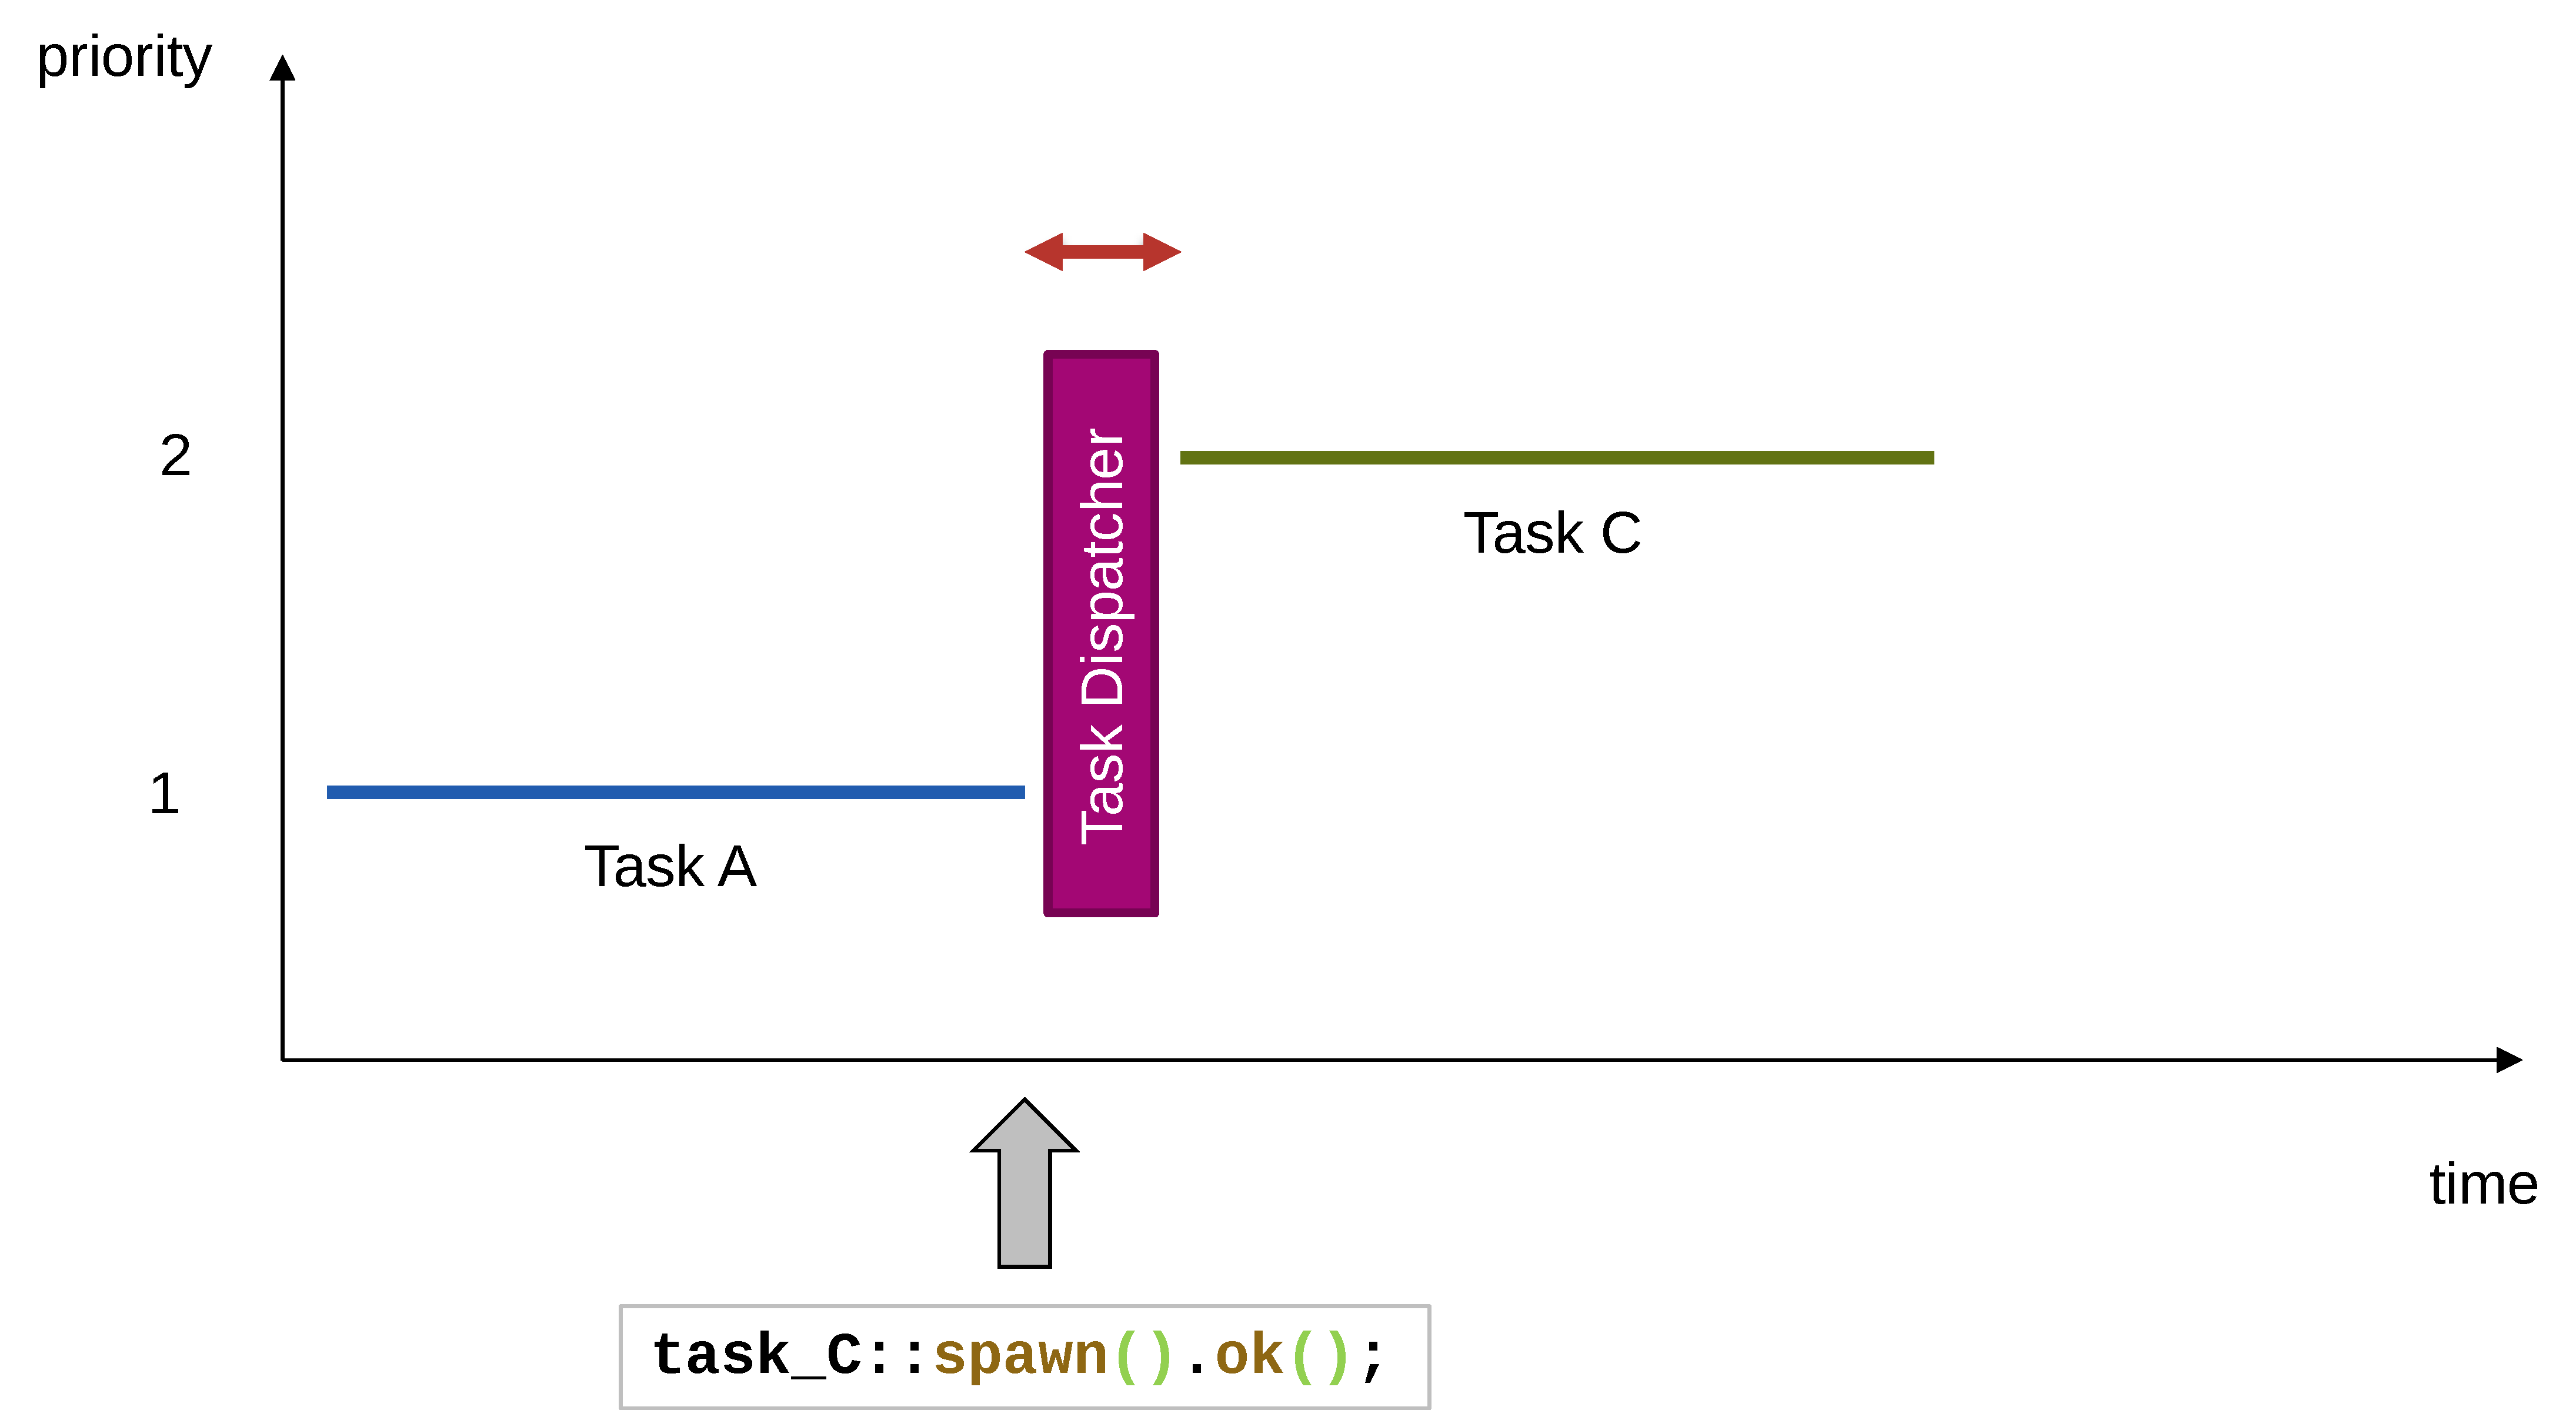
\includegraphics[width=\textwidth]{fig/spawn_prio_high.svg.pdf}
  % Note: We do not have the SVG source file for the image above, so we have to put the PDF under version control.
  \caption{Spawn Task with Higher Priority}%
  \label{fig:spawn_prio_high}
  % Note: The `\label{}` can be on the line after the `\caption{}` if the `\caption{}` line ends with a comment.
\end{figure}

If a task of higher priority (task C) is spawned, the original task is preempted immediately. See figure~\ref{fig:spawn_prio_high}.
We measured the cycles from directly before the execution of the \texttt{task_C::spawn().ok()} statement until the first instruction of the task C Rust function.
This includes the enqueuing of the task into the ready queue of the task dispatcher, the pending of the interrupt associated with the task dispatcher for priority 2, the context switch to the new interrupt handler, the dequeuing of task C, and finally, the prologue of the Rust function of task C.

\subsection{Task Spawn Lower Priority}

\begin{figure}
  \centerfloat
  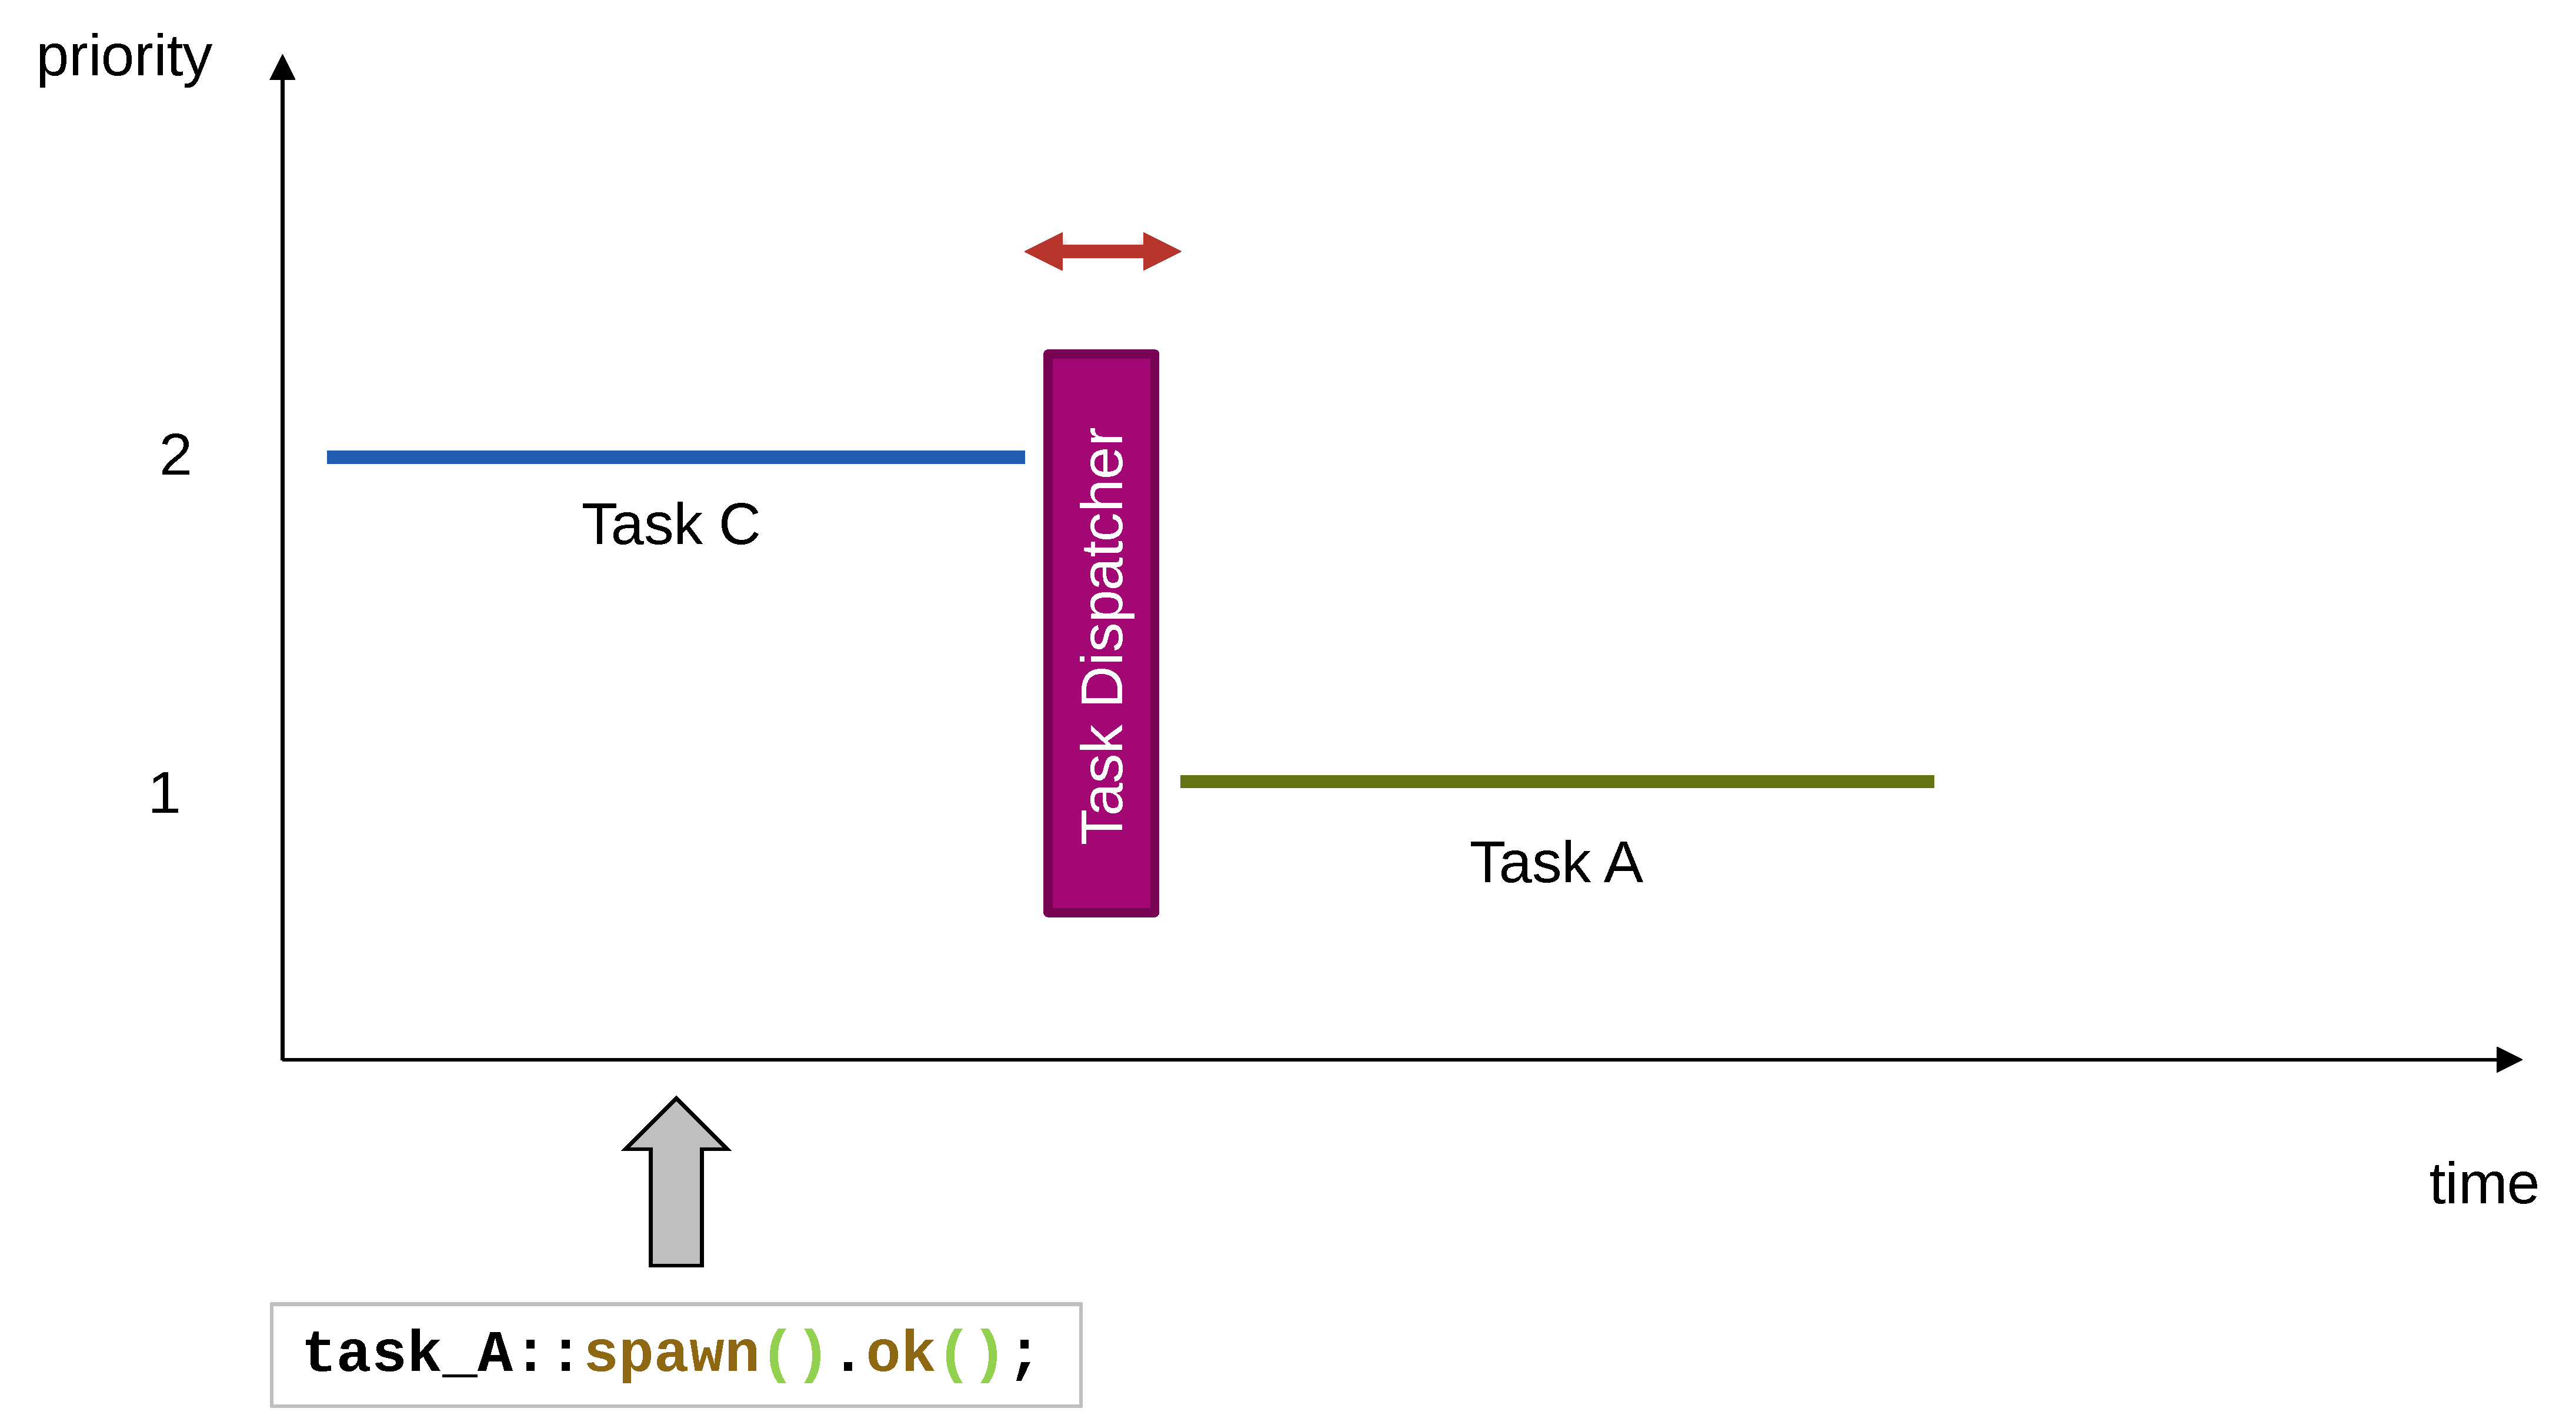
\includegraphics[width=\textwidth]{fig/spawn_prio_low.svg.pdf}
  % Note: We do not have the SVG source file for the image above, so we have to put the PDF under version control.
  \caption{Spawn Task with Lower Priority}%
  \label{fig:spawn_prio_low}
  % Note: The `\label{}` can be on the line after the `\caption{}` if the `\caption{}` line ends with a comment.
\end{figure}

If a task of lower priority is spawned (task A), the new task is enqueued into the ready queue of its task dispatcher, and the corresponding interrupt is pended in software. But since it has lower priority, it does not fire immediately, and the original task (task C) will finish execution first.
In this transition, we measure the cycles between the last instruction of the Rust function of task C and the first instruction of the Rust function of task A. See figure~\ref{fig:spawn_prio_low}.
This includes the epilogue of task C, the interrupt context switch, the dequeuing of task A and the prologue of task A.

\subsection{Task Spawn Equal Priority}

\begin{figure}
  \centerfloat
  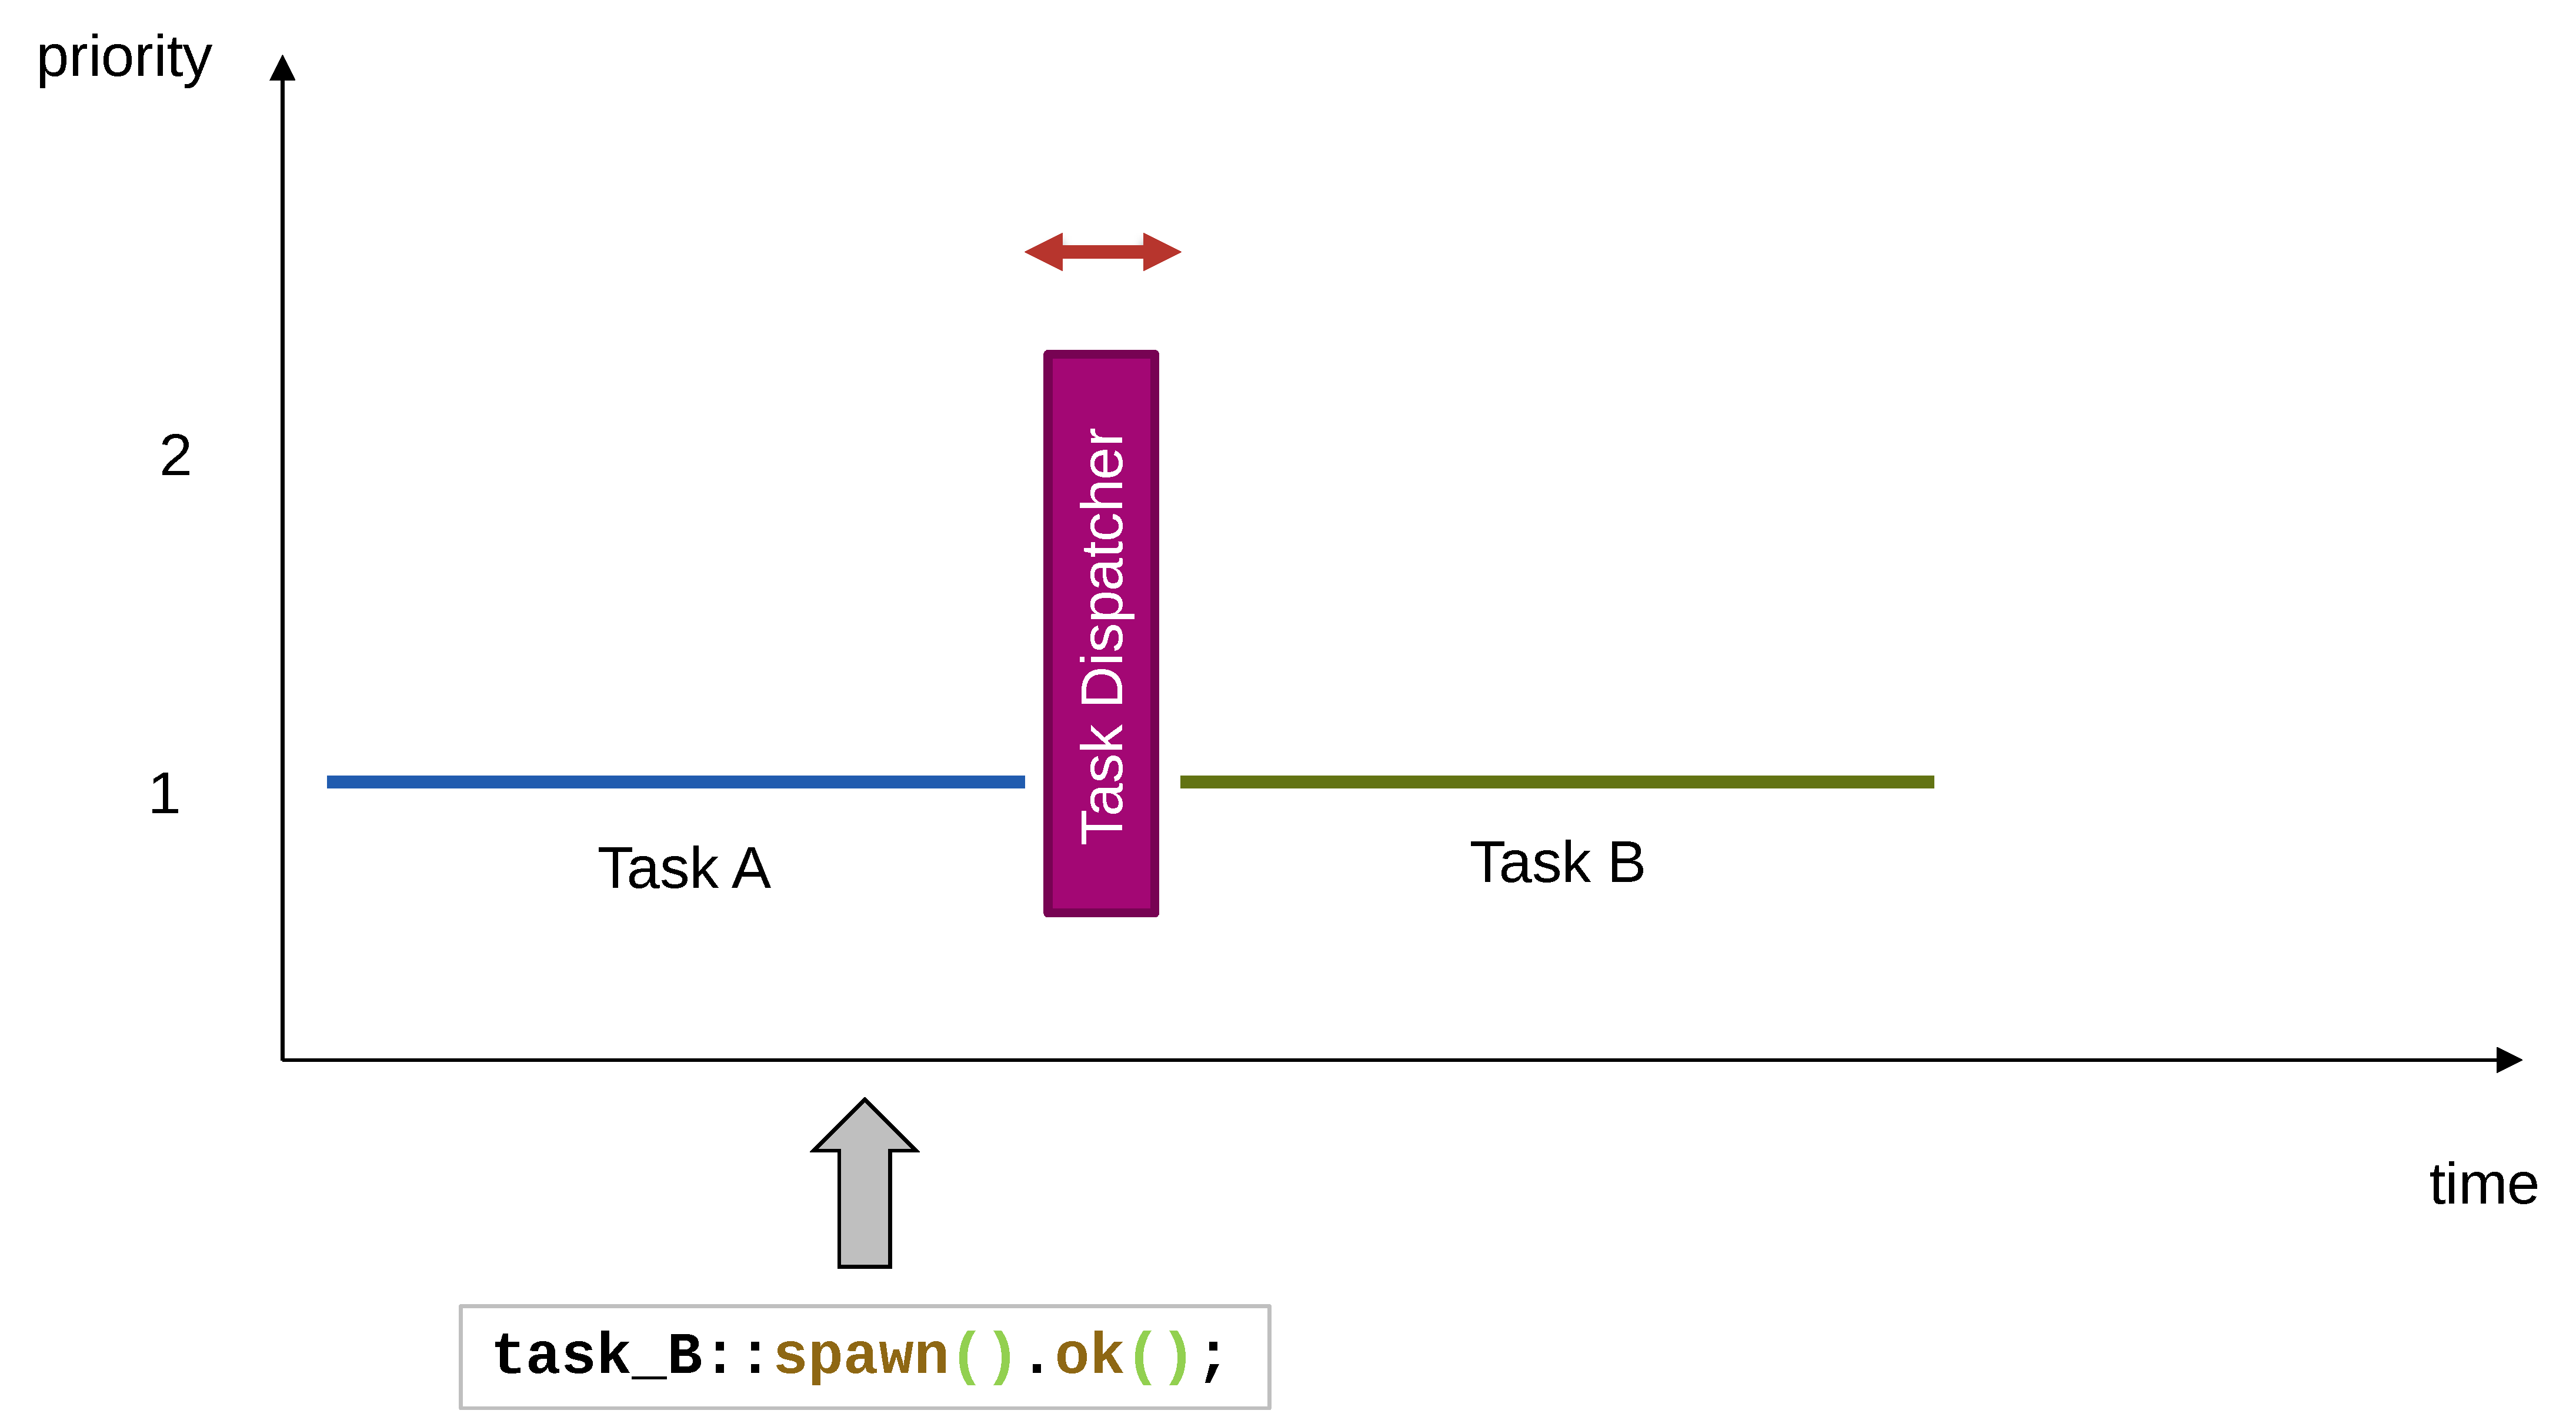
\includegraphics[width=\textwidth]{fig/spawn_prio_equal.svg.pdf}
  % Note: We do not have the SVG source file for the image above, so we have to put the PDF under version control.
  \caption{Spawn Task with Equal Priority}%
  \label{fig:spawn_prio_equal}
  % Note: The `\label{}` can be on the line after the `\caption{}` if the `\caption{}` line ends with a comment.
\end{figure}

If a task of equal priority (task B) is spawned, the new task is enqueued into the ready queue of its task dispatcher, and the corresponding interrupt is pended in software. However, since there is only one task dispatcher per priority, the pended interrupt is actually the same that is currently being handled. This means, that the current task (task A) will run until completion. Then the task dispatcher that is already running will dequeue the new task and run it directly. So no context switch is necessary. Therefore, we measure the number of cycles between the last instruction of task A and the first instruction of task B. See figure~\ref{fig:spawn_prio_equal}.

This includes the epilogue of task A, the dequeuing of task B and the prologue of task B.

\subsection{Timed Task Spawn}

\begin{figure}
  \centerfloat
  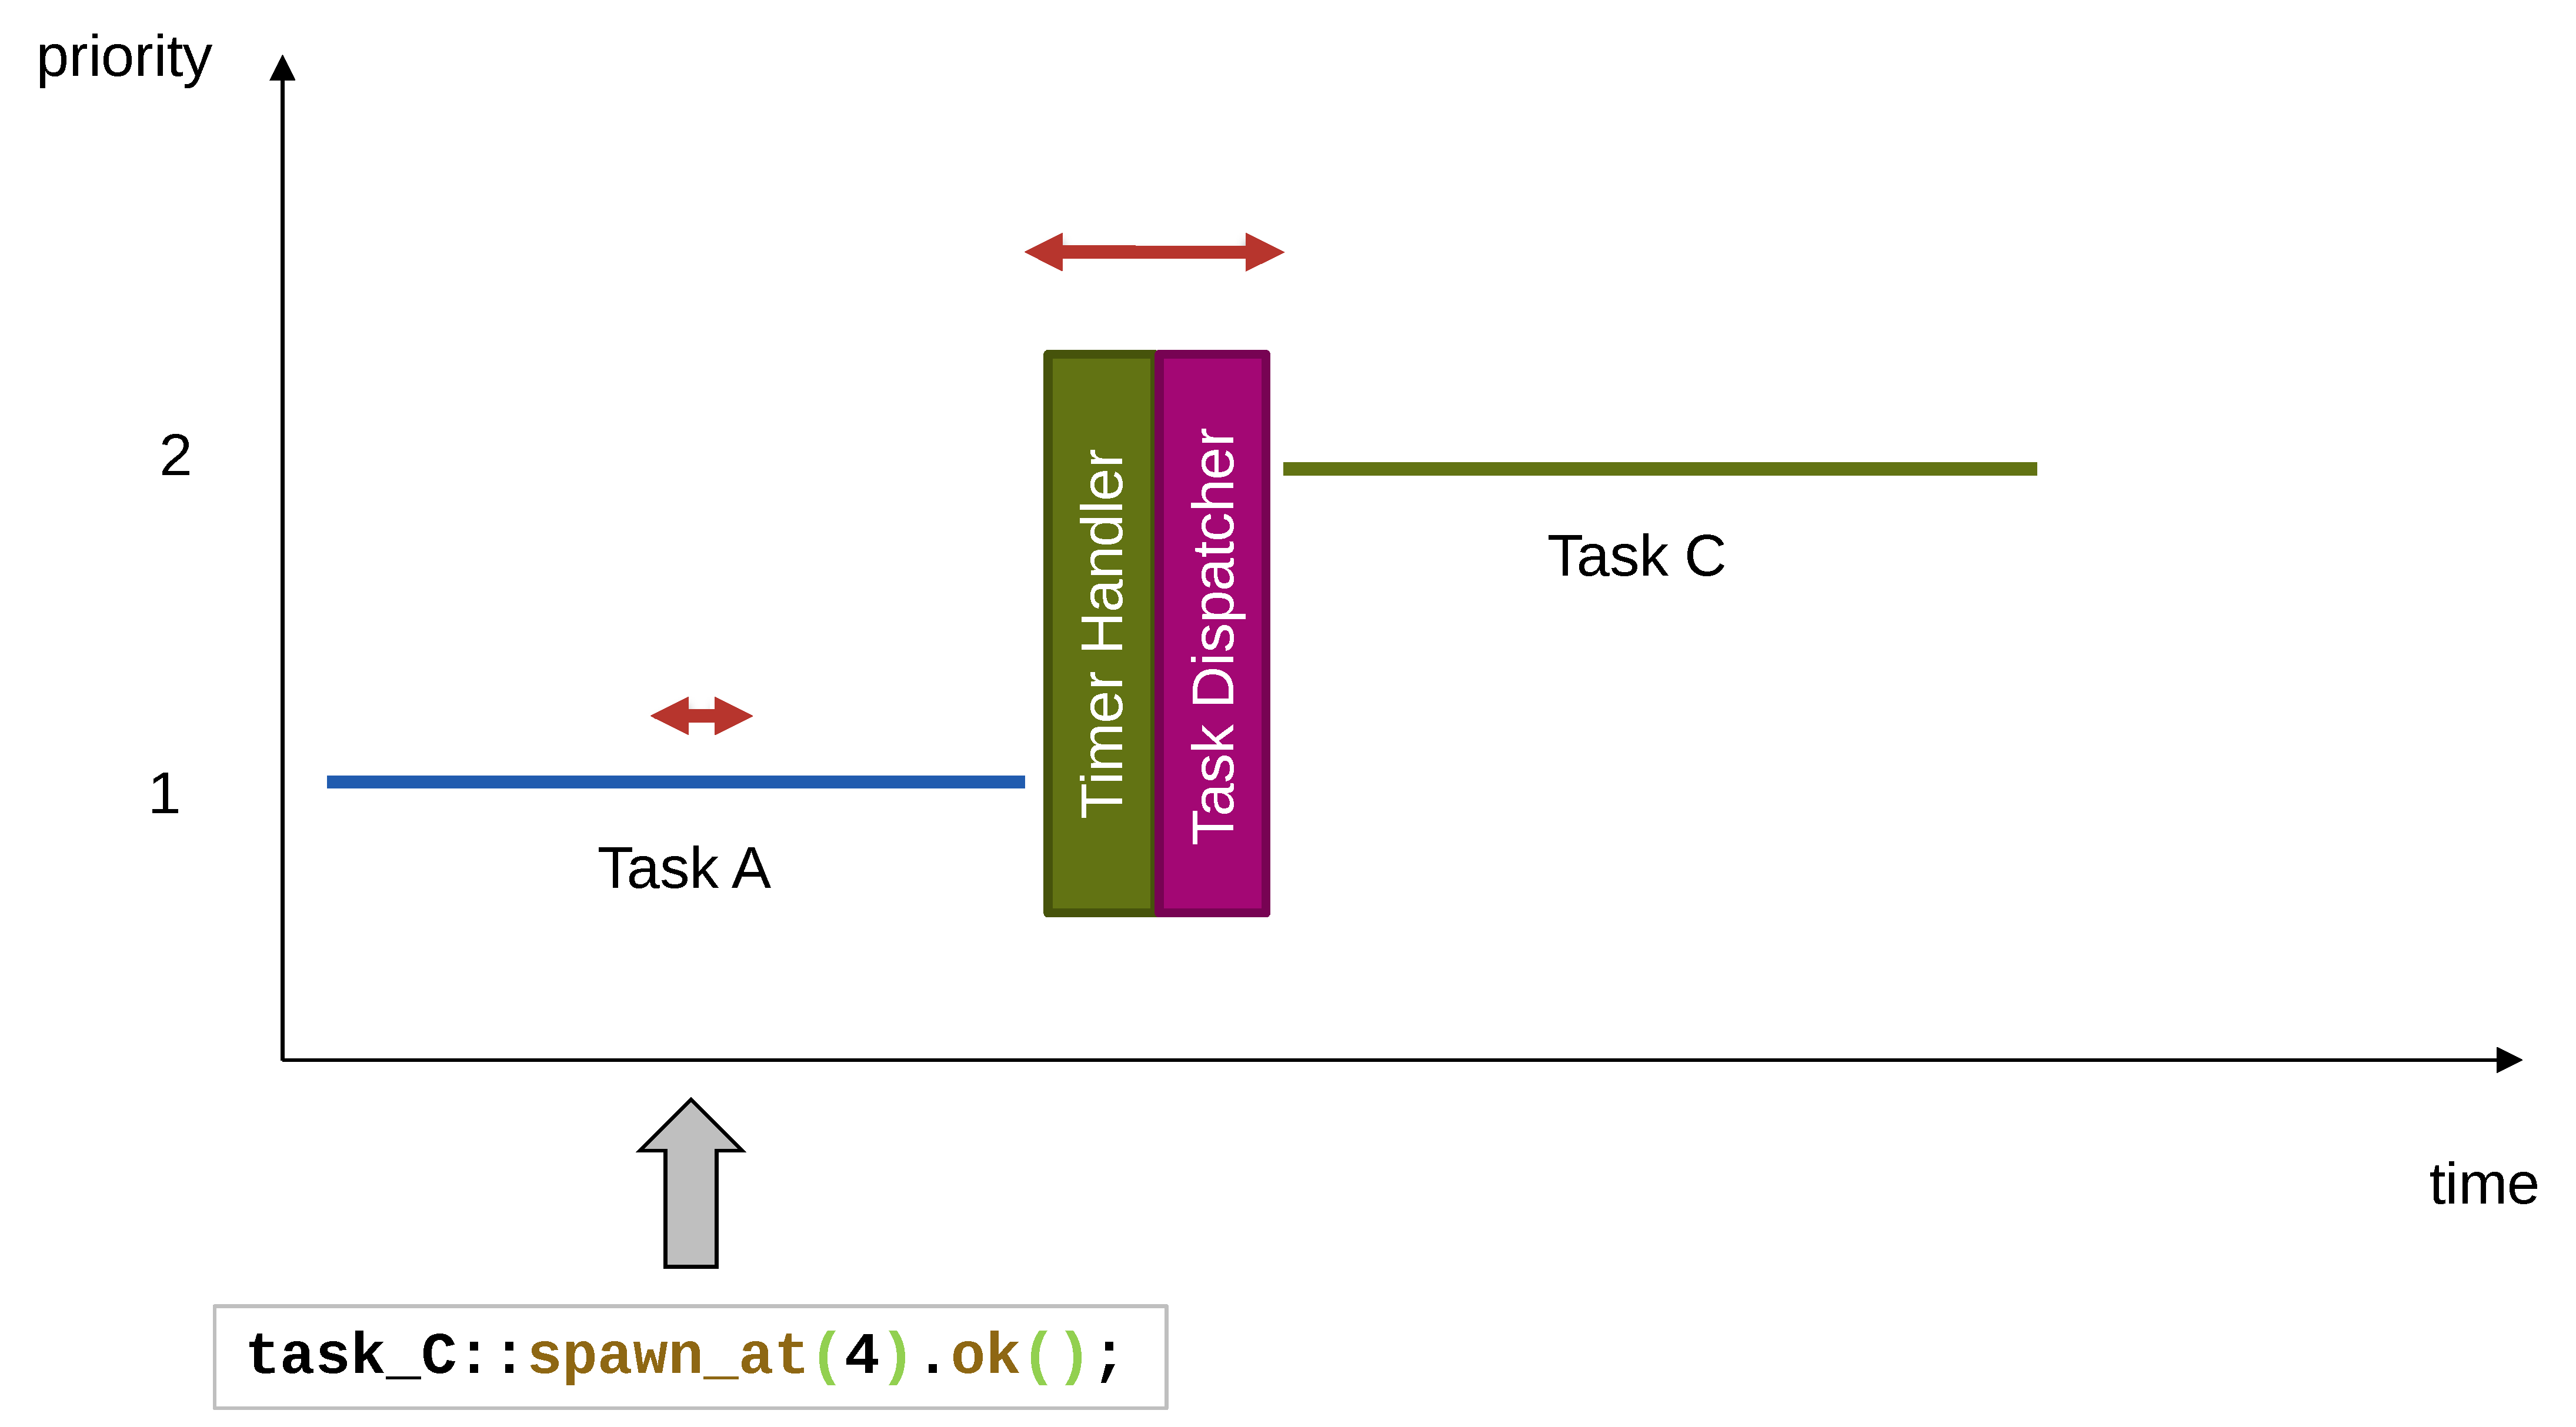
\includegraphics[width=\textwidth]{fig/spawn_prio_timed.svg.pdf}
  % Note: We do not have the SVG source file for the image above, so we have to put the PDF under version control.
  \caption{Spawning of a Timed Task}%
  \label{fig:spawn_prio_timed}
  % Note: The `\label{}` can be on the line after the `\caption{}` if the `\caption{}` line ends with a comment.
\end{figure}

In the spawning process of a timed task (task C), there are two interesting sequences to measure. First, the scheduling of task C. And secondly, the effective start time of task C. See figure~\ref{fig:spawn_prio_timed}.

For the scheduling, the task first is sorted into the timer queue. Then, the timer comparison value is set to the spawn point of the first task in the sorted timer queue. It could actually be finished now, but to catch edge cases, a few safety operations are performed.

Therefore, the timer interrupt is pended, and the context is switched to the timer interrupt. It checks if its first task is already due (which it normally is not, it is only done to catch tasks that are scheduled in the past or very near future), and switches the context back to the original task (task A).

So the cycles between the last instruction before the \texttt{task_C::spawn_at(4).ok} statement and the first instruction after it are measured. This spawning procedure can seam quite inefficient, but it is given by \gls{rtic}.

For the actual starting of task C, we measure the cycles from the point where the timer fires to the first instruction of the Rust function of task C.
This includes the context switch to the timer handler, the dequeuing of task C from the timer queue, the enqueuing of task C into the ready queue of its task dispatcher, the pending of the task dispatcher, the context switch into the task dispatcher's interrupt handler, the dequeuing of task C from the ready queue and finally the prologue of task C.

\subsection{Locking}

Besides the spawning of tasks, sharing resources among tasks is one of the most important processes in operating systems. Therefore, we measure the locking and unlocking overhead of a resource. Since in \gls{rtic} it makes a difference if the locking happens in the task with the highest priority that has access to a specific resource, or in any other task, we measure both cases, see figures~\ref{fig:locking_high_prio} and \ref{fig:locking_low_prio}.

Here, we measure the number of cycles between the last instruction before the locking/unlocking statement and the first instruction after the locking/unlocking statement.

To get a better understanding of how locking of shared resources works in \gls{rtic}, refer to section \ref{sec:shared_resources}.

\begin{figure}
  \centerfloat
  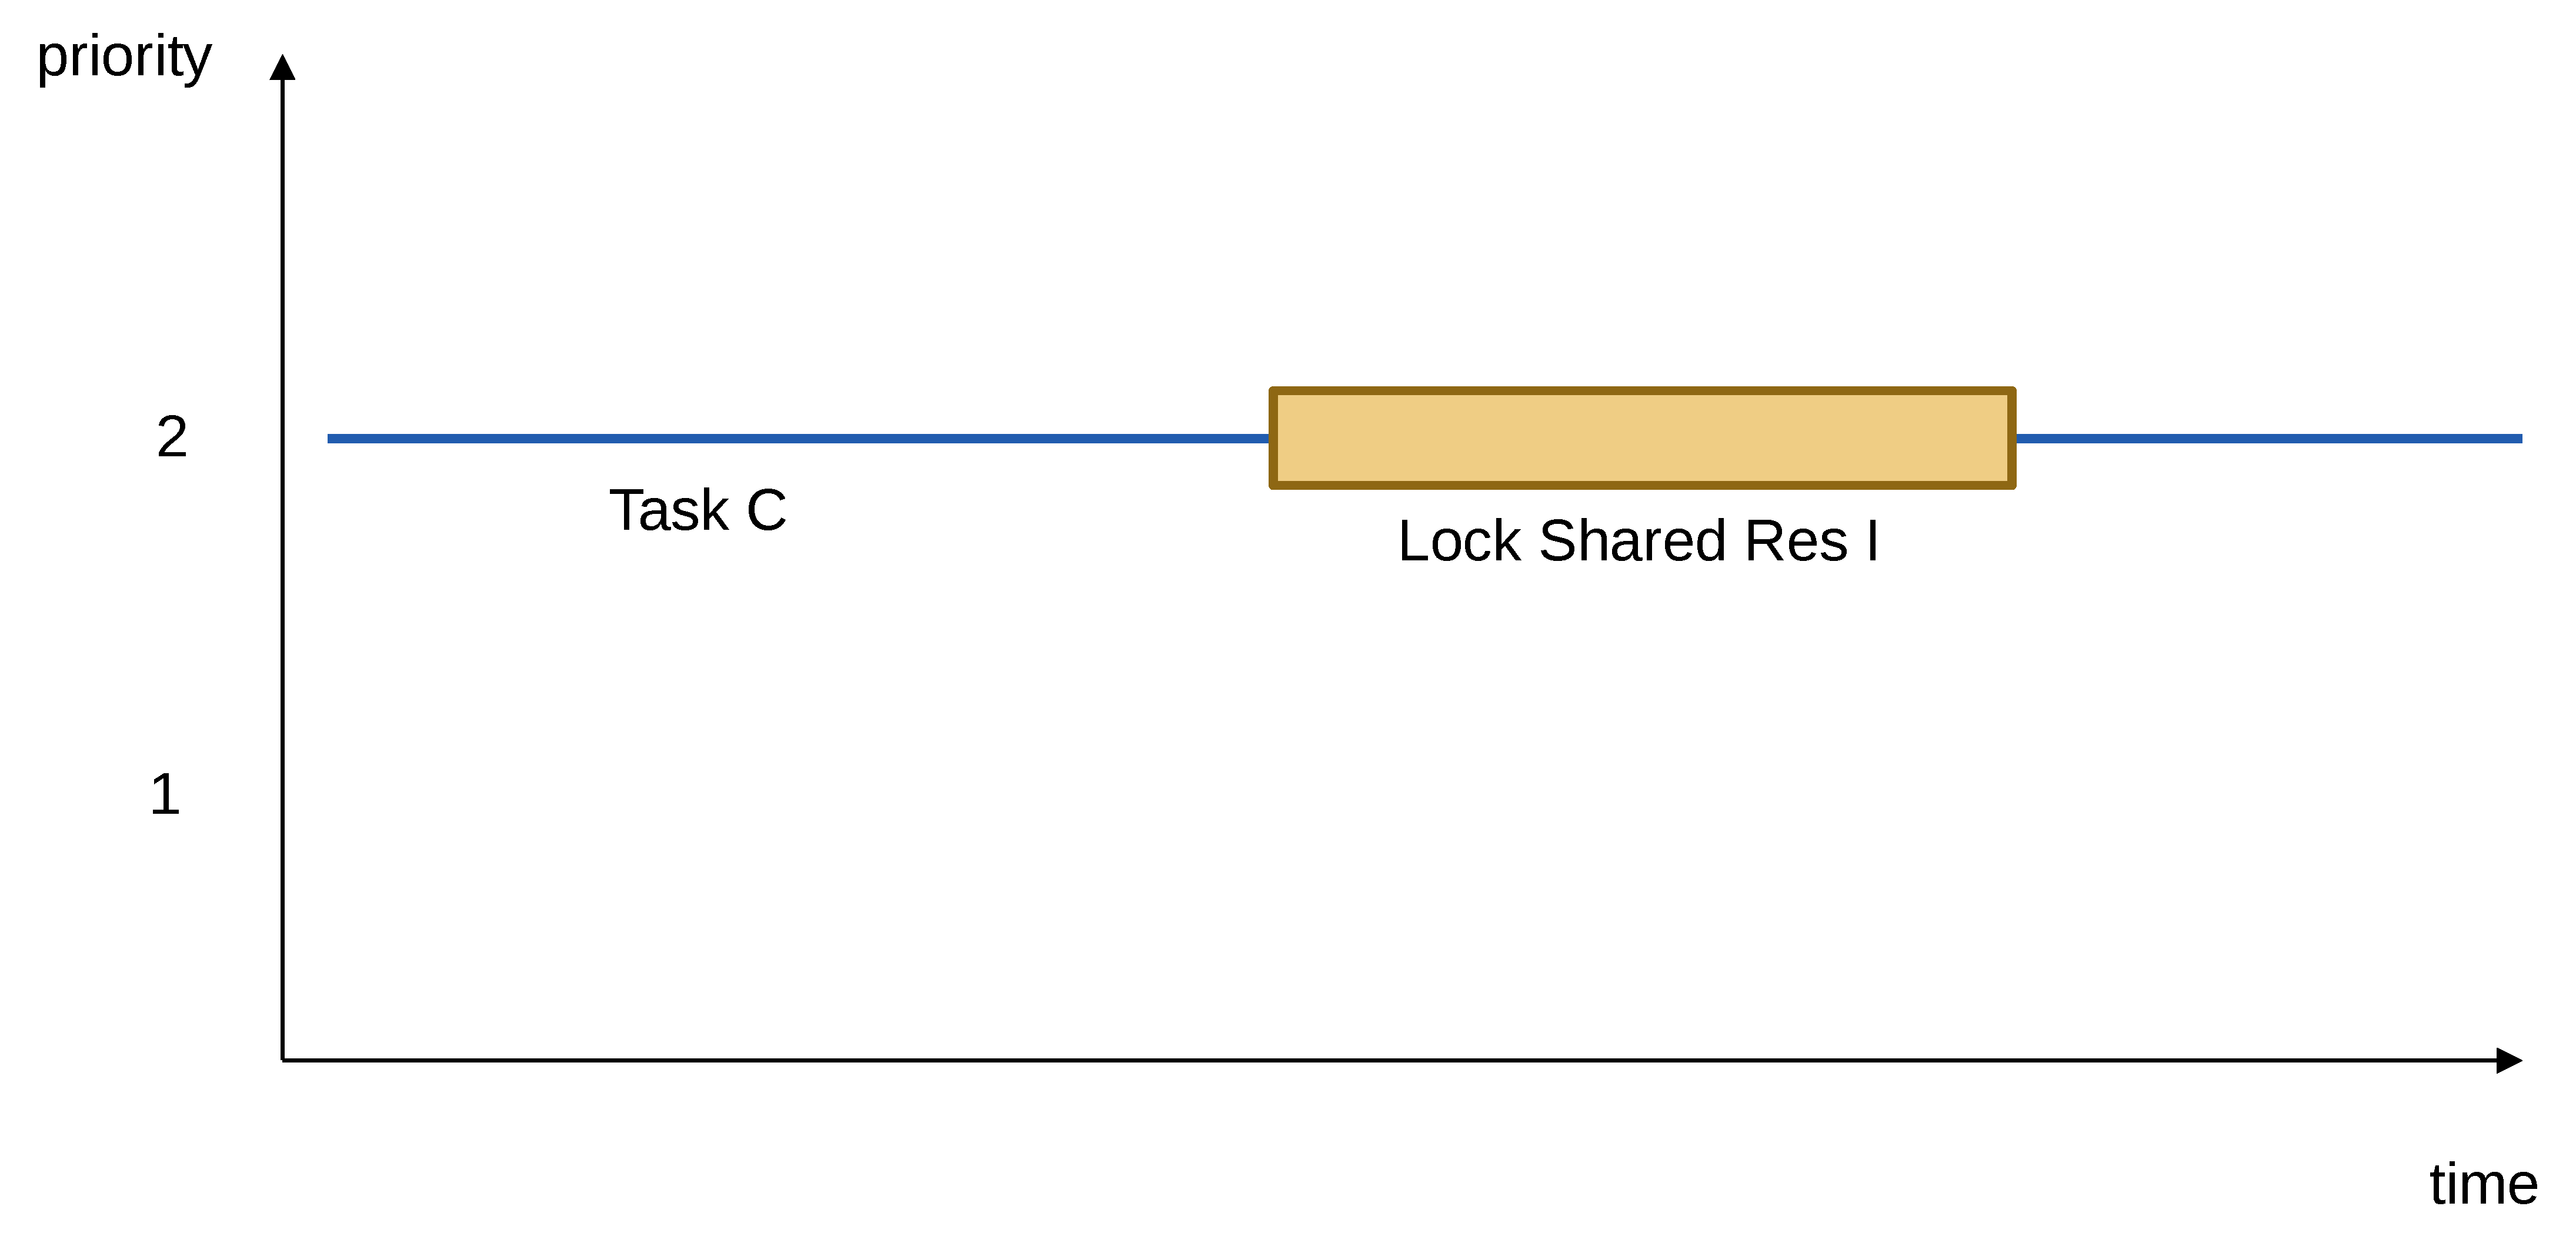
\includegraphics[width=\textwidth]{fig/locking_high_prio.svg.pdf}
  % Note: We do not have the SVG source file for the image above, so we have to put the PDF under version control.
  \caption{Locking of a Resource as highest Priority Task}%
  \label{fig:locking_high_prio}
  % Note: The `\label{}` can be on the line after the `\caption{}` if the `\caption{}` line ends with a comment.
\end{figure}

\begin{figure}
  \centerfloat
  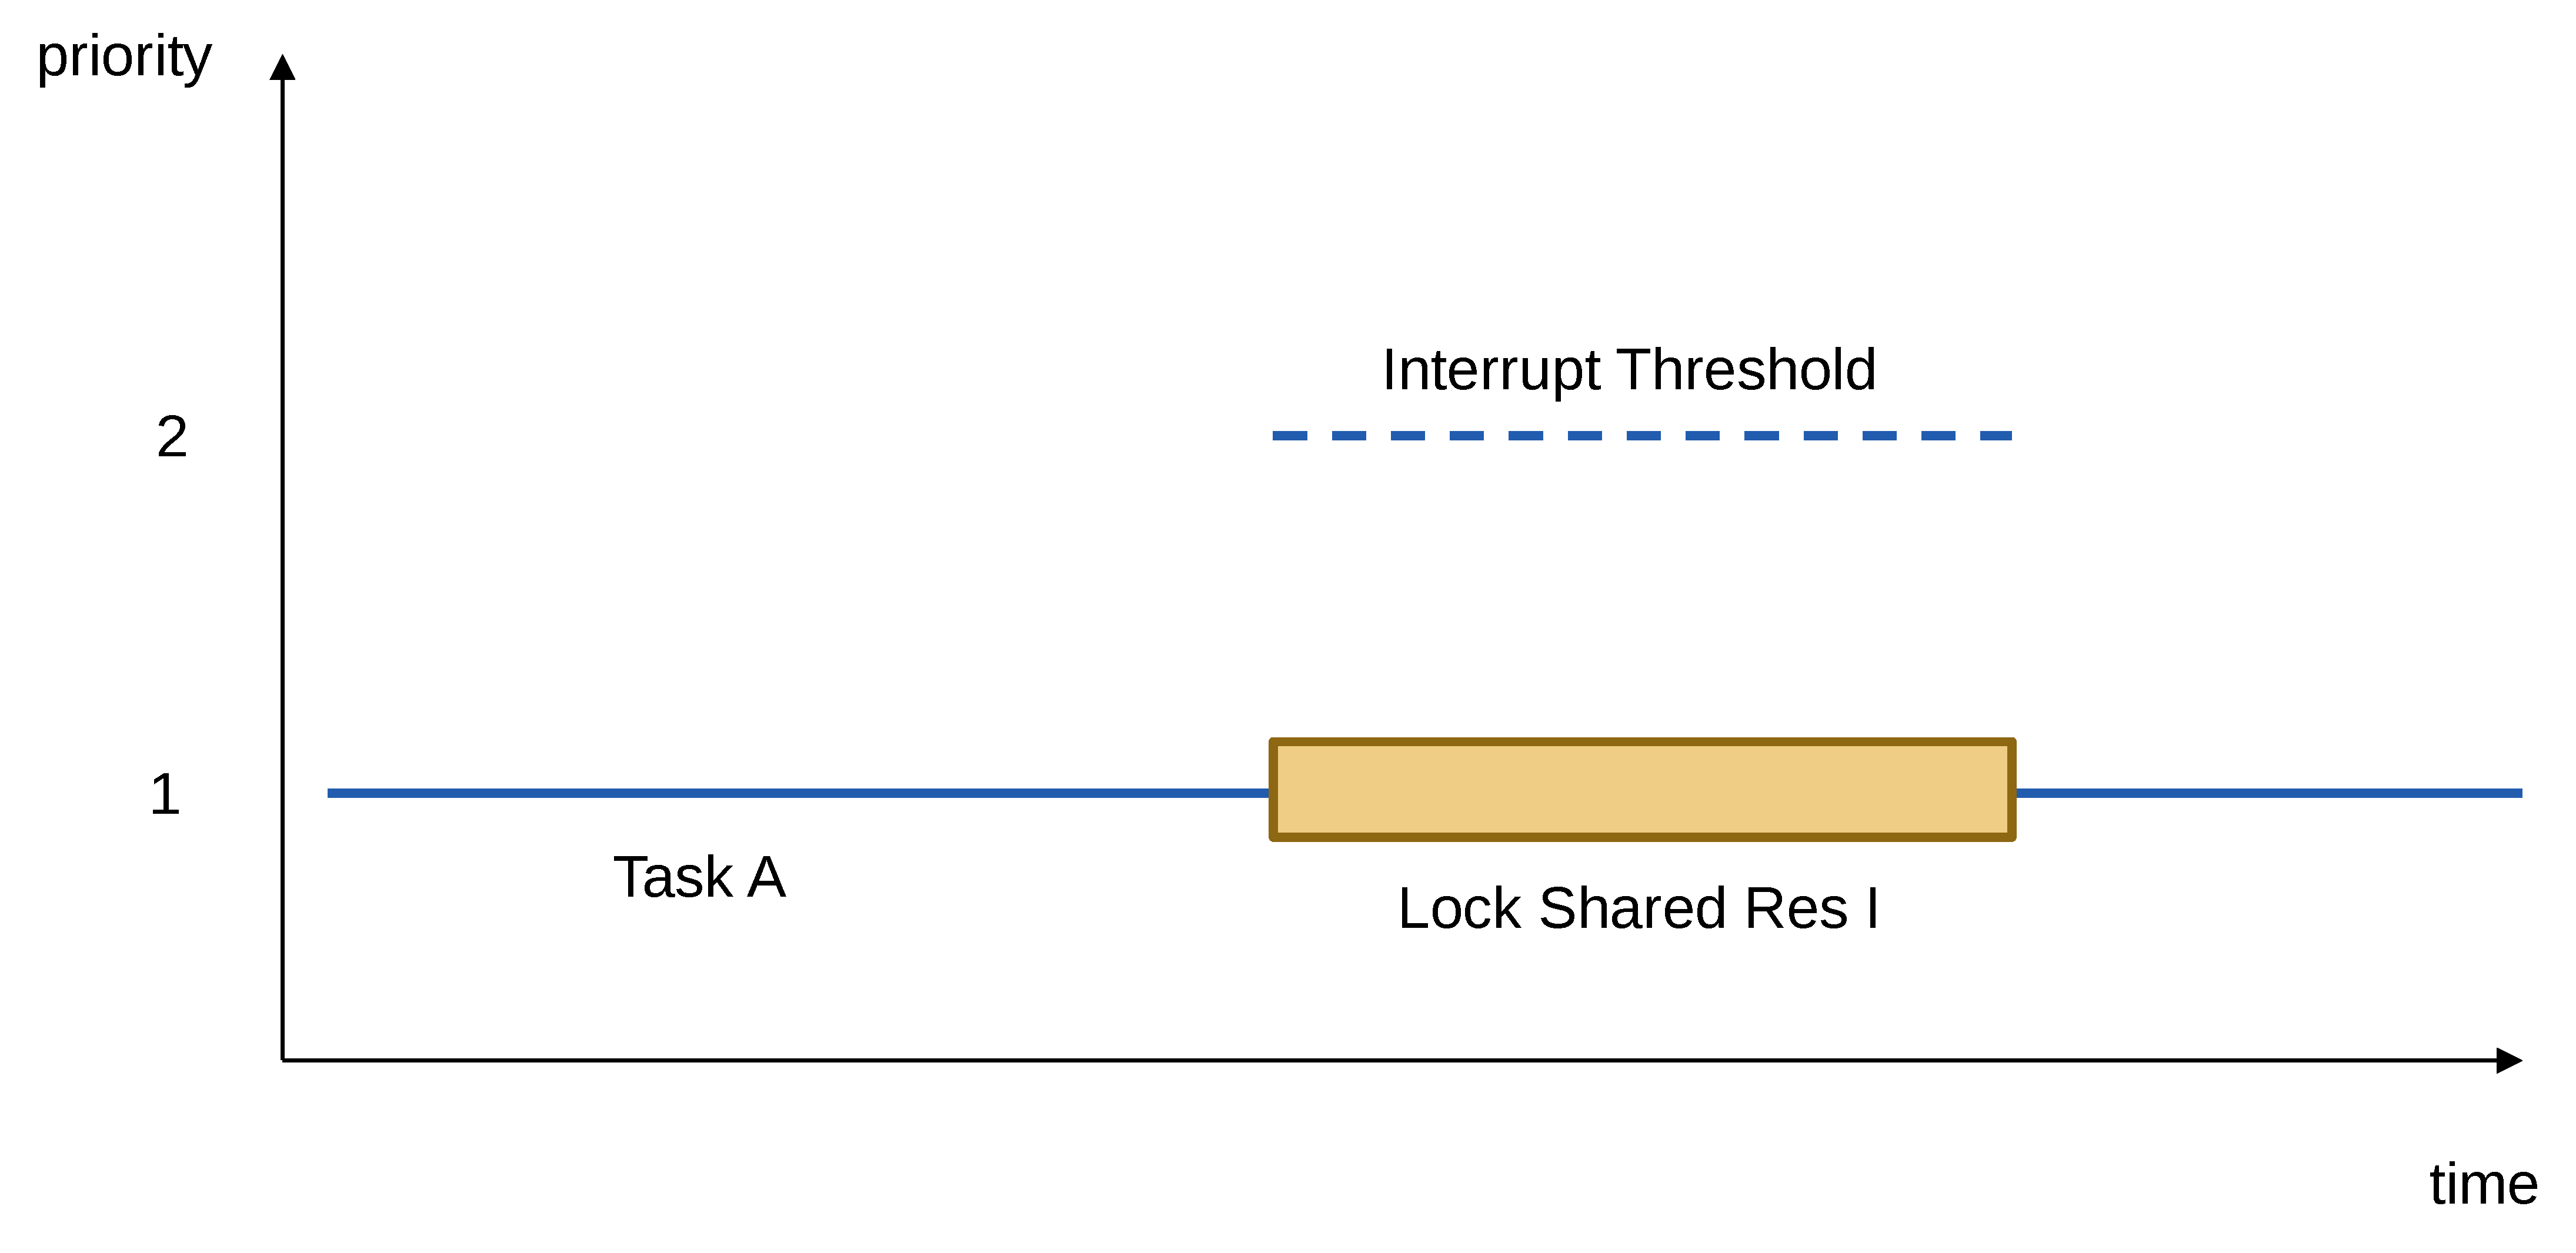
\includegraphics[width=\textwidth]{fig/locking_low_prio.svg.pdf}
  % Note: We do not have the SVG source file for the image above, so we have to put the PDF under version control.
  \caption{Locking of a Resource}%
  \label{fig:locking_low_prio}
  % Note: The `\label{}` can be on the line after the `\caption{}` if the `\caption{}` line ends with a comment.
\end{figure}

\section{Measurement Results}

In the following section, the results of the measurements that are described in section~\ref{sec:core_transitions} are presented.

Since locking of shared resources is already highly optimized by \gls{rtic}, it only uses between about zero and four cycles, which is in the same range as the measurement uncertainties, see section~\ref{sec:time_measurement}. Therefore, we do not show the locking measurements in the plots below, since they do not include any meaningful information.

\subsection{Original Implementation}
\label{sec:results_original_implementation}

In the plot in figure~\ref{fig:plot_original}, one can see the number of cycles that are used by the operations described in section~\ref{sec:core_transitions}. It is clearly visible that the implementation for ARM outperforms the one for RISC-V if the original implementation with the integer ABI is used. The exact cycle count number can be found in table~\ref{tbl:detailed_results}.

We identify two main differences. First, \gls{rtic} needs a 32bit timer for its timer handler. RISC-V already provides this, and therefore no overhead is added. In ARM, however, there exists only a 24bit timer. Therefore, the 32bit functionality had to be added in software. This leads to an overhead and explains why the RISC-V implementation performs better in scheduling timed tasks.

The vastly better performance of the ARM implementation can be explained with the much more performant interrupt handling in ARM. First, it has to be noted, that in ARM, interrupt context switching is handled in hardware, where it is parallelized. In RISC-V however, it is done in software, as explained in section~\ref{sec:interrupt_handler_macro}.

However, we developed hardware and software optimizations for the \gls{clic}.
See sections \ref{sec:results_nxti} and \ref{sec:results_fastirq} for results with an optimized RISC-V setup.


\begin{figure}
\begin{tikzpicture}
\begin{axis}[
	x tick label style={
		/pgf/number format/1000 sep=},
	ylabel=Cycle Count,
	enlargelimits=0.05,
	legend style={at={(0.5,1.1)},
	anchor=north,legend columns=-1},
        ybar=0cm,
        xtick=data,
        %xmajorgrids=true,
        width=\textwidth,
        enlarge x limits={abs=0.8},
        xticklabels={Hardware Task, Higher Prio Task, Equal Prio Task , Lower Prio Task, Scheduling Timed Task, Start Timed Task},
        xticklabel style={rotate=45, anchor=east},
]
\addplot [draw=none,fill=ETHBlue]
	coordinates {(0,32) (1,143)
		 (2,43) (3,106) (4,322) (5,332)};
\addplot [draw=none,fill=ETHRed]
	coordinates {(0,58) (1,170)
		 (2,51) (3,178) (4,307) (5,372)};
\legend{Arm Cortex-M3 eabi,rv32imac}
\end{axis}
\end{tikzpicture}
\caption{Performance of Original Implemenation}
\label{fig:plot_original}
\end{figure}


\subsection{NXTI}
\label{sec:results_nxti}

ARM uses a technology that is called \emph{tail-chaining}. It is used to skip unnecessary context switches. The same behavior can be achieved by using the NXTI \gls{csr} of the \gls{clic} as described in section~\ref{sec:nxti}.

By using it, context switches between cascading interrupts can be avoided. They appear when a lower priority task is spawned, or a timed task starts. In figure~\ref{fig:plot_nxti} it can be seen, that the performance is comparable to ARM in both transitions.

See table~\ref{tbl:nr_of_context_switches} for the number of necessary context saves and restorations per core transition. It shows the values for the original implementation as well as for the case where NXTI is used.

The other transitions, however, still suffer from the slow context switch in RISC-V, as explained in section~\ref{sec:results_original_implementation}.

See section~\ref{sec:results_fastirq} for further optimizations.

\begin{figure}
\begin{tikzpicture}
\label{fig:plot_nxti}
\begin{axis}[
	x tick label style={
		/pgf/number format/1000 sep=},
	ylabel=Cycle Count,
	enlargelimits=0.05,
	legend style={at={(0.5,1.1)},
	anchor=north,legend columns=-1},
        ybar=0cm,
        xtick=data,
        %xmajorgrids=true,
        width=\textwidth,
        enlarge x limits={abs=0.8},
        xticklabels={Hardware Task, Higher Prio Task, Equal Prio Task , Lower Prio Task, Scheduling Timed Task, Start Timed Task},
        xticklabel style={rotate=45, anchor=east},
]
\addplot [draw=none,fill=ETHBlue]
	coordinates {(0,32) (1,143)
		 (2,43) (3,106) (4,322) (5,332)};
\addplot [draw=none,fill=ETHRed]
	coordinates {(0,58) (1,170)
		 (2,51) (3,178) (4,307) (5,372)};
\addplot [draw=none,fill=ETHPurple]
	coordinates {(0,60) (1,172)
		 (2,51) (3,116) (4,326) (5,329)};
\legend{Arm Cortex-M3 eabi,rv32imac,rv32imac (nxti)}
\end{axis}
\end{tikzpicture}
\caption{Performance with Usage of NXTI}
\end{figure}

\subsection{\texttt{fastirq}}
\label{sec:results_fastirq}

Since context switches in ARM are handled in parallel in hardware, they are much more performant than the standard RISC-V software solution.

In the implementation described in section~\ref{sec:context_switch}, a context switch statically takes 27 cycles. There exists a hardware extension for RISC-V, called \texttt{fastirq}, that enables a saving and restoring context in the background while the interrupt handler Rust function can already start its execution. The whole context switch delay is therefore reduced to 8 cycles. This is a static improvement of 19 cycles per context switch.

Due to time constraints, this hardware extension could not be added to the evaluation setup, however, since all improvements are statically, an accurate estimation can easily be performed. The results of this estimation are shown in figure~\ref{fig:plot_fastirq}.

In both transitions where timers are involved, RISC-V beats ARM by far, for the reasons explained in section~\ref{sec:results_original_implementation}. In general, ARM still performs slightly better than RISC-V. Further improvements are discussed in section~\ref{sec:future_work}.


\begin{figure}
\begin{tikzpicture}
\label{fig:plot_fastirq}
\begin{axis}[
	x tick label style={
		/pgf/number format/1000 sep=},
	ylabel=Cycle Count,
	enlargelimits=0.05,
	legend style={at={(0.5,1.1)},
	anchor=north,legend columns=-1},
        ybar=0cm,
        xtick=data,
        %xmajorgrids=true,
        width=\textwidth,
        enlarge x limits={abs=0.8},
        xticklabels={Hardware Task, Higher Prio Task, Equal Prio Task , Lower Prio Task, Scheduling Timed Task, Start Timed Task},
        xticklabel style={rotate=45, anchor=east},
]
\addplot[draw=none,fill=ETHBlue]
	coordinates {(0,32) (1,143)
		 (2,43) (3,106) (4,322) (5,332)};
\addplot [draw=none,fill=ETHRed]
	coordinates {(0,58) (1,170)
		 (2,51) (3,178) (4,307) (5,372)};
\addplot  [draw=none,fill=ETHPurple]
	coordinates {(0,60) (1,172)
		 (2,51) (3,116) (4,326) (5,329)};
\addplot[ETHBlue,pattern=north east lines, pattern color=ETHBlue20]
	coordinates {(0,41) (1,153)
		 (2,51) (3,116) (4,288) (5,310)};
\legend{Arm Cortex-M3 eabi,rv32imac,rv32imac (nxti),rv32imac (fastirq) estimation}
\end{axis}
\end{tikzpicture}
\caption{Performance Estimation with E-Extension and EABI}
\end{figure}


\begin{table}
  \centerfloat
  \begin{tabular}{ l r r r r }
    \toprule
    Transition & Arm Cortex-M3 eabi & rv32imac & rv32imac (nxti) & rv32imac (fastirq) estimation \\
    \midrule
    Hardware Task & 32 & 58 & 60 & 41\\
    Higher Prio Task & 143 & 170 & 172 & 153 \\
    Equal Prio Task & 43 & 51 & 51 & 51\\
    Lower Prio Task & 106 & 178 & 116 & 116\\
    Scheduling Timed Task & 322 & 307 & 326 & 288\\
    Start Timed Task & 332 & 372 & 329 & 310 \\
    \bottomrule
  \end{tabular}
  \caption{Cycle Count per Core Transition}%
  \label{tbl:detailed_results}
\end{table}

\begin{table}
  \centerfloat
  \begin{tabular}{ l r r r r }
    \toprule
    Transition & Saves & Restorations & Saves (nxti) & Restorations (nxti) \\
    \midrule
    Hardware Task & 1 & 0 & 1 & 0\\
    Higher Prio Task & 1 & 0 & 1 & 0 \\
    Equal Prio Task & 0 & 0 & 0 & 0 \\
    Lower Prio Task & 1 & 1 & 0 & 0\\
    Scheduling Timed Task & 1 & 1 & 1 & 1\\
    Start Timed Task & 2 & 1 & 1 & 0 \\
    \bottomrule
  \end{tabular}
  \caption{Number of Context Switches}%
  \label{tbl:nr_of_context_switches}
\end{table}